%%%%%%%%%%%%%%%%%%%%%%%%%%%%%%%%%%%%%%%%%%%%%%%%%%%%%%%%%%%%%%%%%%%%%%
% How to use writeLaTeX:
%
% You edit the source code here on the left, and the preview on the
% right shows you the result within a few seconds.
%
% Bookmark this page and share the URL with your co-authors. They can
% edit at the same time!
%
% You can upload figures, bibliographies, custom classes and
% styles using the files menu.
%
% If you're new to LaTeX, the wikibook is a great place to start:
% http://en.wikibooks.org/wiki/LaTeX
%
%%%%%%%%%%%%%%%%%%%%%%%%%%%%%%%%%%%%%%%%%%%%%%%%%%%%%%%%%%%%%%%%%%%%%%
\documentclass{tufte-handout}

%\geometry{showframe}% for debugging purposes -- displays the margins

\usepackage{amsmath}

% Set up the images/graphics package
\usepackage{graphicx}
\setkeys{Gin}{width=\linewidth,totalheight=\textheight,keepaspectratio}
\graphicspath{{graphics/}}

\title{Hands-On Session: Data Encryption}
\author{DIME Analytics \\ dimeanalytics@worldbank.org}
\date{11 June 2019}  % if the \date{} command is left out, the current date will be used

% The following package makes prettier tables.  We're all about the bling!
\usepackage{booktabs}

% The units package provides nice, non-stacked fractions and better spacing
% for units.
\usepackage{units}

% The fancyvrb package lets us customize the formatting of verbatim
% environments.  We use a slightly smaller font.
\usepackage{upquote}
\usepackage{fancyvrb}
\fvset{fontsize=\normalsize}
\renewcommand{\FancyVerbFormatLine}{\color{violet}}
\DefineShortVerb{\|}

% Small sections of multiple columns
\usepackage{multicol}

% Provides paragraphs of dummy text
\usepackage{lipsum}

% Allows clickable links
\usepackage[colorlinks = true,
linkcolor = blue,
urlcolor  = blue,
citecolor = blue,
anchorcolor = blue]{hyperref}

% These commands are used to pretty-print LaTeX commands
\newcommand{\doccmd}[1]{\texttt{\textbackslash#1}}% command name -- adds backslash automatically
\newcommand{\docopt}[1]{\ensuremath{\langle}\textrm{\textit{#1}}\ensuremath{\rangle}}% optional command argument
\newcommand{\docarg}[1]{\textrm{\textit{#1}}}% (required) command argument
\newenvironment{docspec}{\begin{quote}\noindent}{\end{quote}}% command specification environment
\newcommand{\docenv}[1]{\textsf{#1}}% environment name
\newcommand{\docpkg}[1]{\texttt{#1}}% package name
\newcommand{\doccls}[1]{\texttt{#1}}% document class name
\newcommand{\docclsopt}[1]{\texttt{#1}}% document class option name

\begin{document}

\maketitle% this prints the handout title, author, and date

\begin{marginfigure}%
  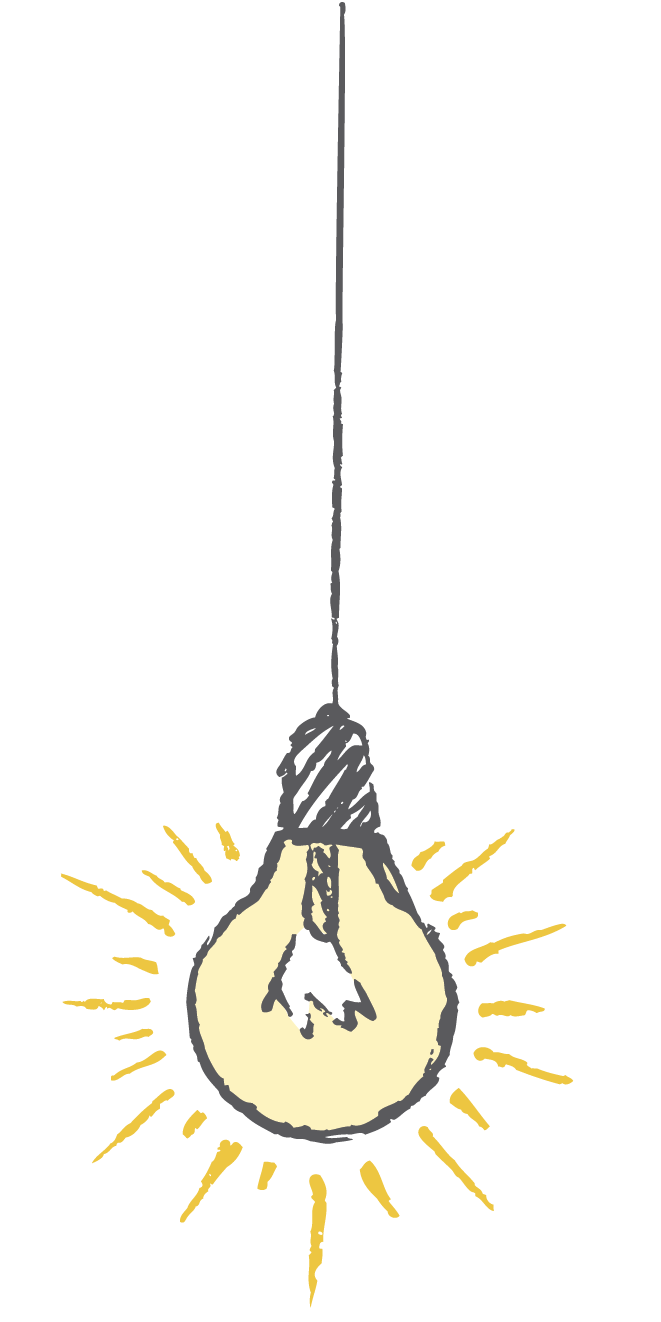
\includegraphics[width=\linewidth]{img/light.png}
\end{marginfigure}

\begin{abstract}
In this exercise we will encrypt a dataset and attempt to access the data in an encrypted folder

\bigskip\noindent \textbf{Exercise Objectives}: On completing this exercise you will be able to
\begin{enumerate}
  \item Set up VeraCrypt
  \item Encrypt files
  \item Access encrypted files
\end{enumerate}
\end{abstract}

%\printclassoptions
\section{Part 1: Set up VeraCrypt}

First we will install VeraCrypt. Note that this needs to be done only once. Anyone accessing a file encrypted using VeraCrypt requires the software installed on their computer.

\begin{enumerate}
	\item Install \href{https://www.veracrypt.fr/en/Downloads.html}{Veracrypt}. (eServices request on a Bank desktop/laptop)
	\item Create an encrypted folder (volume) titled 'Encrypted Data' with a strong password.\sidenote{Add suggestions for how to make strong passwords} \\
	\textit{Note that, you can use any drive of your choice.}\sidenote{Add sub-steps for this (maybe with pictures)}
	\begin{itemize}
		\item  Click Create Volume (marked with a red rectangle for clarity)
	\end{itemize}
	\begin{figure}%
		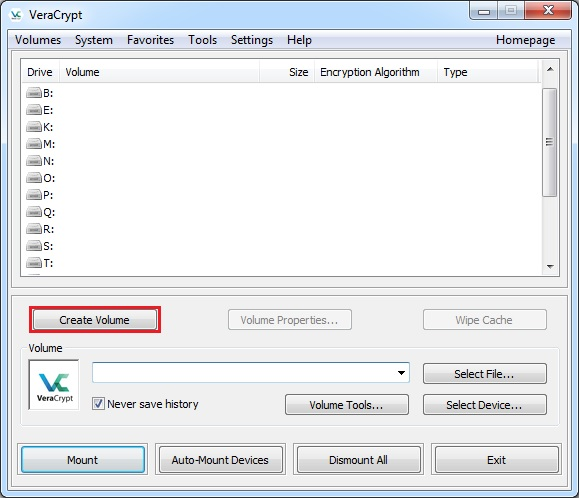
\includegraphics[width=\linewidth]{img/vc_install_1.png}
	\end{figure}
	\begin{itemize}
	\item  The VeraCrypt Volume Creation Wizard window should appear.
	In this step you need to choose where you wish the VeraCrypt volume to be created.In this session, we will choose the first option and create a VeraCrypt volume within a file.
	\end{itemize}
	\begin{figure}%
		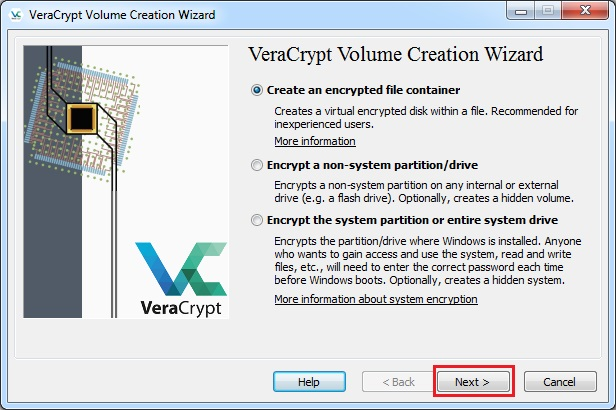
\includegraphics[width=\linewidth]{img/vc_install_2.png}
	\end{figure}
	\begin{itemize}
		\item  In this step you need to choose whether to create a standard or hidden VeraCrypt volume. In this tutorial, we will choose the former option and create a standard VeraCrypt volume.
	\end{itemize}
	\begin{figure}%
		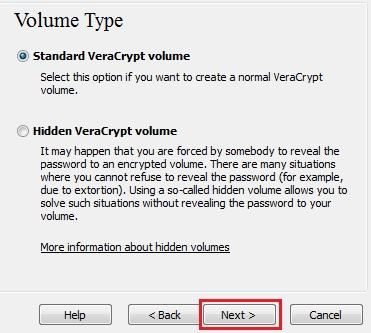
\includegraphics[width=\linewidth]{img/vc_install_3.png}
	\end{figure}
	\begin{itemize}
		\item  In this step you have to specify where you wish the VeraCrypt volume (file container) to be created. Note that a VeraCrypt container is just like any normal file. It can be, for example, moved or deleted as any normal file. It also needs a filename, which you will choose in the next step.  Click Select File.
	\end{itemize}
	\begin{figure}%
		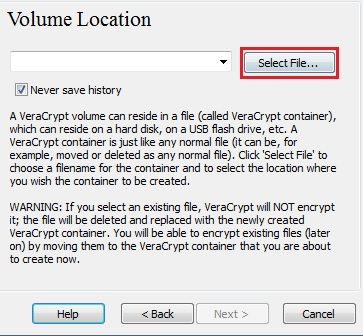
\includegraphics[width=\linewidth]{img/vc_install_4.png}
	\end{figure}
	\begin{itemize}
		\item  Select the desired path (where you wish the container to be created) in the file selector. Type the desired container file name in the Filename box.
	Click Save.
	\end{itemize}
	\begin{figure}%
		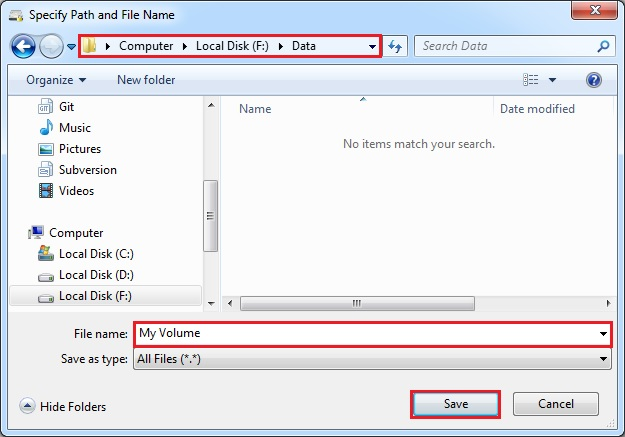
\includegraphics[width=\linewidth]{img/vc_install_5.png}
	\end{figure}
	\begin{itemize}
		\item  In the Volume Creation Wizard window, click Next.
	\end{itemize}
	\begin{figure}%
		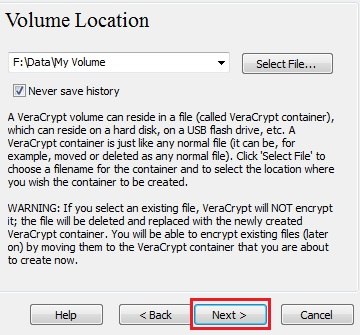
\includegraphics[width=\linewidth]{img/vc_install_6.png}
	\end{figure}
	\begin{itemize}
		\item  Here we specify that we wish the size of our VeraCrypt container to be 250 megabyte. You may, of course, specify a different size. After you type the desired size in the input field (marked with a red rectangle), click Next.
	\end{itemize}
	\begin{figure}%
		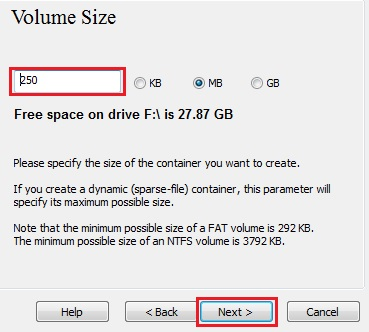
\includegraphics[width=\linewidth]{img/vc_install_7.png}
	\end{figure}
	\begin{itemize}
		\item  This is one of the most important steps. Here you have to choose a good volume password. Read carefully the information displayed in the Wizard window about what is considered a good password.
		After you choose a good password, type it in the first input field. Then re-type it in the input field below the first one and click Next.
	\end{itemize}
	\begin{figure}%
		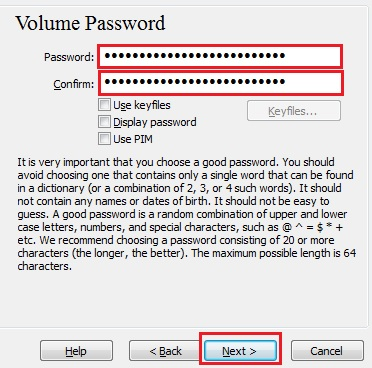
\includegraphics[width=\linewidth]{img/vc_install_8.png}
	\end{figure}
	\begin{itemize}
		\item  Move your mouse as randomly as possible within the Volume Creation Wizard window at least until the randomness indicator becomes green. The longer you move the mouse, the better (moving the mouse for at least 30 seconds is recommended). This significantly increases the cryptographic strength of the encryption keys (which increases security).
		Click Format.
	\end{itemize}
	\begin{figure}%
		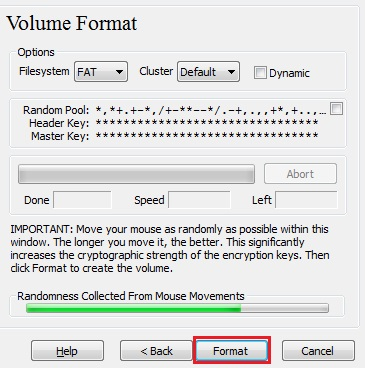
\includegraphics[width=\linewidth]{img/vc_install_9.png}
	\end{figure}

		\item Go to the location where you created the folder to confirm the folder exists.
	Double click on the folder to try and open it directly. Confirm that it doesn't open!
\end{enumerate}

%\printclassoptions
\section{Part 2: Encrypting files}
\begin{enumerate}
	\item Open VeraCrypt.
	\item Mount the encrypted volume created onto drive K. \\
	\textit{Note that, you can use any drive of your choice.}
	\item This will now open an empty folder titled 'Encrypted Data'. Save a copy of the data sets titled endline\_data\_raw\_2018.dta and endline\_data\_raw\_nodup\_2018.dta\sidenote{Update to final dataset once ready} in the folder. \\
	\textit{This is very similar to using a new USB/flash drive and adding files to it.}
	\item Open VeraCrypt and dismount the drive.
	\item Share the password securely with team members.\sidenote{Add something about securely sharing passwords}
	
\end{enumerate}


%\printclassoptions
\section{Part 3: Access encrypted files}
\begin{enumerate}
	\item Open VeraCrypt.
	\item Mount the encrypted volume created onto drive K. \\
	\textit{Note that, you can use any drive of your choice.}
	\item This will now open a folder titled 'Encrypted Data' which contains the data sets titled endline\_data\_raw\_2018.dta and endline\_data\_raw\_nodup\_2018.dta\sidenote{Update to final dataset once ready}.
	\item Open VeraCrypt and dismount the drive   
\end{enumerate}

NOTE: When calling a file in the encrypted folder on Stata the file path used will be that of the mounted drive and not that of where the encrypted file is stored. 
Example: Encrypted folder is stored in Dropbox at\sidenote{add pictures to explain}. It will be used in Stata using mounted drive and not the filepath of the Dropbox folder. add stata example on file path for mounted drive, but do not worry about doing it in the big master dofile
\section{Extra - If time permits}
Pair up with another person in the room and try to create, share, and access encrypted data.
\begin{enumerate}
	\item Create a shared Dropbox/Box/Onedrive folder.
	\item Create one encrypted folder for each of you within this shared folder.
	\item Place the data in your folder in that shared folder.
	\item Share the password with partner
	\item Access partner's encrypted file
\end{enumerate}

\end{document}
